\chapter*{Forward}\label{chap:forward}
\addcontentsline{toc}{chapter}{\nameref{chap:forward}}


\begin{quote}
All truths are easy to understand once they are discovered; the point is to discover them.
\emph{(Source:  Galileo Galilei, ``Dialogue on the Two Chief World Systems'')}
\end{quote}

\section*{To the student:}\label{sec:toStudent}
\addcontentsline{toc}{section}{\nameref{sec:toStudent}}

\medskip

Many students start out liking math. Some like it well enough that they even want to teach it. However, when they reach advanced math classes (such as abstract algebra), they become bewildered and frustrated. Their textbooks talk about strange mathematical thingamabobs they've never heard of, which have nonsensical properties that come from who knows where. In lectures, the professor/oracle  makes pronouncements (a.k.a ``theorems'') and utters long incantations (a.k.a ``proofs'') , but it's hard to see the point of either. 
\medskip

If the above paragraph describes you, then this book is meant for you!
\medskip

There's a good reason why higher math classes are bewildering for most students. I believe that we math instructors tend to take too much for granted.\footnote{My father always says that trying to understand math is frustrating, but once you've got it it's even more frustrating to try to explain it to others.} It's easy to forget that we're only able to understand abstractions because we have concrete examples that we keep referring back to, consciously or subconsciously. These examples enable us to fit new abstract ideas in with specific behaviors and patterns that we're very familiar with. But students who don't have a firm hold on the examples have nothing to hold on to, and are left grasping (and gasping) for air. 

To be sure, most students have previously been exposed to various important examples that historically gave rise to abstract algebra. These examples include the complex numbers, integers mod $n$, symmetries, and so on. They can give definitions and do some basic computations according to the rules. But they haven't been given a chance to internalize these examples.  They can kind of follow along, but they aren't ``fluent".

Our hope is that after reading this book students will be able to say, ``I've seen complex numbers, integers mod $n$ and permutations before, but now I understand what makes them tick. I can see they have  deep underlying similarities, which they share with other mathematical structures.'' 

This is actually a very good time to be learning abstract algebra. Abstract algebra hs moved from the outer boondocks inhabited by specialists and puzzle enthusiasts out  into the center stage of modern  science and technology. Two areas where abstract algebra has made strong contributions stand out particularly: information processing and physics. Coding of information is at the heart of information technology, and abstract algebra provides all of the methods of choice for information coding that is both reliable (impervious to errors) and private.  
On the other hand,  many if not most of the great advances in  physics in the past 100 years are due to deeper understanding of physical symmetries and the groups that produce them (the Lorentz group in special relativity is just one example). We try as much as possible to make connections with these two areas, and hope to do so increasingly in future editions. 

We hope you enjoy the book. Send us your comments!

\section*{To the instructor}\label{sec:toInstructor}
\addcontentsline{toc}{section}{\nameref{sec:toInstructor}}

This book  is not intended for budding mathematicians. It was created for a math program in which most of the students in upper-level math classes are planning to become secondary school teachers. For such students, conventional abstract algebra texts are practically  incomprehensible, both in style and in content. Faced with this situation, we decided to create a book that our students could actually read for themselves. In this way we have been able to dedicate class time to problem-solving and personal  interaction rather than rehashing the same material in lecture format.

In our program, the book was used in a 2-semester sequence of courses. The first semester dealt with the important foundational examples: complex  and modular numbers (with applications to cryptography), summation and polynomials, as well as review of sets and functions.  The second semester began with symmetries and permutation groups (the archtypical examples of finite groups) to lead the student into basic group theory. Doubtless other math prgrams will take very different approaches, and instructors are welcome to customize the text as per their individual needs. Instructors may gain access to the \LaTeX  source by emailing \href{mailto:thron@tamuct.edu}{thron@tamuct.edu}. 

The book is highly modular, and chapters may be readily omitted if students are already familiar with the material. Some chapters  (``Preliminaries'' and ``Sigma Notation'') are remedial. Other chapters cover topics that are often covered in courses in discrete mathematics, such as sets, functions, and equivalence classes. (Much of this material is taken from the Morris' book, with some amplifications.) We have found from experience that students need this re-exposure in order to gain the necessary facility with these concepts, on which so much of the rest of the book is based.

Admittedly the material falls short of the typical syllabus for an upper-level abstract algebra class. But what's the point of covering the syllabus, if the students don't retain anything?  The unhappy fact is that many students at this level haven't yet mastered the important basic examples (complex numbers, etc.) that provide motivation, so it's unrealistic to expect them to grasp abstractions if they don't even understand what's being abstractified.So instead we have dived deeply into the basic examples that will be most useful to students who plan to become secondary educators. Whenever possible we have introduced applications, which may be omitted at the instructor's discretion. We feel that it is critically important for preparing secondary teachers to be familiar with these applications, which they will remember  long after they've forgotten all the theoretical proof stuff. The chapters related to cryptography and coding theory may also be useful for students interested in electrical engineering. 



\section*{Additional resources}\label{sec:additionalResources}
\addcontentsline{toc}{section}{\nameref{sec:additionalResources}}
\
This is the Information Age, and a mere textbook is somewhat limited in its ability to convey information.  Accordingly, as we continue to use the book in our classes, we are continuing to build an ecosystem  to support the book's use:
\begin{itemize}
\item
The book's web site is \url{http://abstractalgebra.altervista.org/}.
\item
An electronic version of the book is available at \url{https://sl2x.aimath.org/book/aafmt/}.
\item
For a print copy, we recommend an on-demand print service such as \url{https://www.printme1.com/}.
\item
 A comprehensive set of short video presentations of the book's content may be found on the EAAEA YouTube channel: \url{https://www.youtube.com/playlist?list=PL2uooHqQ6T7PW5na4EX8rQX2WvBBdM8Qo}. A second YouTube channel with worked exercises may be found at: \url{https://www.youtube.com/playlist?list=PL2uooHqQ6T7NMO1Lk5lX3tDyQF8URCwwK}. 
\item
An \term{Instructor's Supplement}\index{Solutions to exercises}  is available upon request. The supplement contains solutions to most (but not all) exercises, as well as some example test questions.  To obtain the supplement,  email the editor \href{mailto:thron@tamuct.edu}{thron@tamuct.edu} from a verifiable faculty email address.
\item
Any instructor wishing to customize the material or extract certain portions may email the editor \href{mailto:thron@tamuct.edu}{thron@tamuct.edu}  to request the \LaTeX~source code. 
\end{itemize}


\medskip

\noindent
\section*{Acknowledgements}\label{sec:ack}
\addcontentsline{toc}{section}{\nameref{sec:ack}}

In our preparation of this text, we were fortunate to find via the web  some extraordinarily generous authors (Tom Judson, Dave Witte Morris and Joy Morris, A. J. Hildebrand) who freely shared their material with us. Thanks to them, we were able to put the first version of this  textbook together within the span of a single semester (not that we're finished -- this is a living book, not a dead volume). We hope that other instructors will similarly benefit from the material offered here.  

Several Master's students at Texas A\&M-Central Texas have made contributions to the book as part of a projects course or thesis. Their names are listed in the title, and their contributions are acknowleged at the beginning of each chapter. The ``Study Guides'' at the end of the early chapters are written by Katrina Smith. 

Our very special thanks to Meghan DeWitt for her thorough critical reading of the book and her incisive comments. The book has greatly benefitted from her numerous suggestions.
\medskip 

\begin{quote}
Unless the LORD builds the house, the builders labor in vain. Unless the LORD keeps the city, the watchman is wakeful in vain.  It is vanity to rise up early, stay up late, and eat the bread of sorrows, for He gives sleep to those He loves."  (Psalm 127:1-2)
\end{quote}

\chapter*{Organization plan of the book}\label{chap:Org}
\addcontentsline{toc}{chapter}{\nameref{chap:Org}}
A chapter organization diagram is given in Figure~\ref{fig:organization}. Brief descriptions of the chapters and their dependencies are as follows:
\begin{figure}[htb]
	   \center{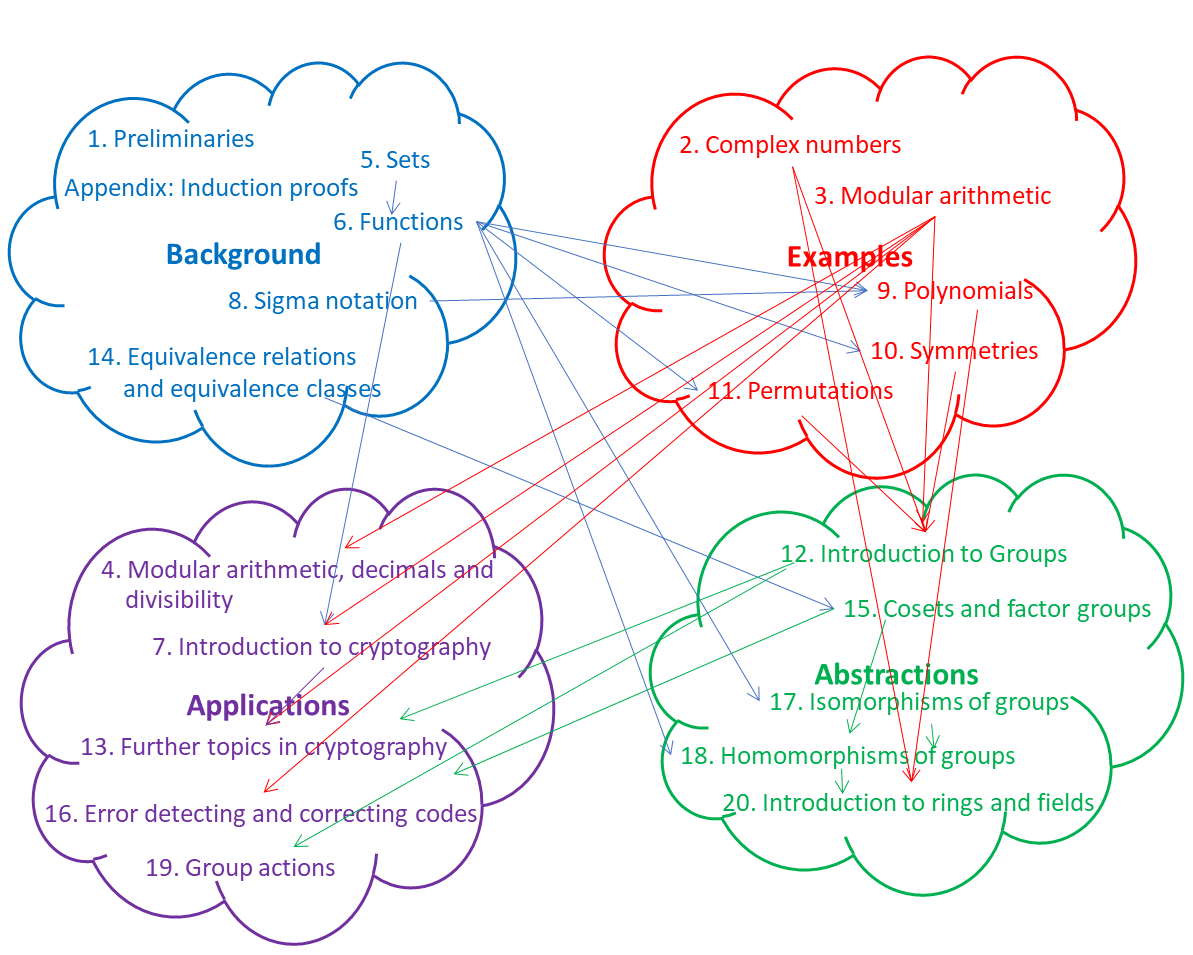
\includegraphics[width=1.1\textwidth]
	         {images/chapterDependence.png}}
	  \caption{\label{fig:organization} Interdependence of chapters}
\end{figure}

\begin{enumerate}
\item
Preliminaries: A review of properties of integers, rationals, and reals, at the high school level. We only review the properties—we do not formally construct these number systems. Some remedial exercises are included.  Used in: All other chapters.
\item
Complex numbers: Basic properties of complex arithmetic, polar form, exponentiation and roots. Some exercises require proofs of complex number properties.  The last section presents applications to signal processing and fractals. Used in: Symmetries (10); all theory chapters (  
\item
Modular arithmetic:  ${\mathbb Z}_n$ is the  gold-standard example for finite groups and rings.  Arithmetic properties, Euclidean algorithm, Diophantine equations; We bring out homomorphism properties (without the terminology).  Used in: all subsequent chapters
\item
Modular arithmetic, decimals, and divisibility: application of modular arithmetic to decimal representation of real numbers (in arbitrary bases) and divisibility rules. 
\item
Sets.  Basic set properties. Can be skipped if students have an adequate background in discrete math. Used in: functions
\item
Functions. Basic ideas of domain, range, into, onto, bijection.  This chapter can be skipped if students have an adequate background.  Used in: all subsequent chapters
\item
Introduction to cryptography:  Explains the concepts of public and private key cryptography, and describes some classic cyphers as well as RSA. Used in:  Further topics in Cryptography (13)
\item
Sigma notation: This chapter prepares for the “polynomials” chapter.  Sigma notation is useful in linear algebra as well. Can be skipped if students are already familiar with this notation. Used in: Polynomials (9) 
\item
Polynomials: fundamental example of rings. Euclidean algorithm for polynomials over fields. FTOA, prove easy part and discuss the hard part.  Will cover this again more rigorously in later chapter. Used in:  Introduction to Groups (12), Introduction to Rings (20)
\item
Symmetries: Symmetries are a special case of permutations. They are treated first because they are easily visualizable, and because they connect algebraic aspects to geometry as well as complex numbers.  Used in:  Permutations (11)
\item
Permutations: In light of Cayley’s theorem, this example is key to the understanding of finite groups. Students are introduced to the mechanics of working with permutations, including cycle multiplication. Cycle structure is explored, as are even and odd permutations. Used in:  Introduction to Groups (12)
\item
Introduction to Groups: This chapter introduced basic properties of groups, subgroups, and cyclic groups, drawing heavily on the examples presented in previous chapters. Used in:  all subsequent chapters
\item
Further topics in cryptography.  Diffie-Hellman key exchange, elliptic curve cryptography over ${\mathbb R}$ and over ${\mathbb Z}_p$
\item
Equivalence relations and equivalence classes. This material is necessary for understanding cosets. This chapter may be skipped if studentshave seen them before.  Used in:  Cosets and Factor Groups (15)
\item
Cosets and Factor Groups: Introductory properties, Lagrange’s theorem, Fermat’s Theorem, simple groups.  Used in: all subsequent chapters.
\item
Error Detecting and Correcting Codes. A discussion of block codes. Some knowledge of linear algebra is required.
\item
Isomorphisms of Groups: Examples and basic properties; direct products (internal and external); classification of abelian groups up to isomorphism. Used in: all subsequent chapters
\item
Homomorphisms of Groups: Kernel of homomorphism; properties; first isomorphism theorem.  Used in: all subsequent chapters
\item
Group Actions: Besides basic definitions, this chapter contains a long discussion of group actions applied to regular polyhedral, as well as the universal covering space of the torus.
\item
Introduction to Rings:  Includes definitions and examples; subrings and product rings; extending polynomial rings to fields;  isomorphisms and homomorphisms; ideals; principal ideal domains; prime ideals and unique factorization domains; division rings; fields;  algebraic extensions. 
\item
Appendix: Induction Proofs—patterns and examples.  Some proofs in the book require induction. This section gives the background needed for students to write formal induction proofs. 
\end{enumerate}

\chapter*{Glossary of Symbols}\label{glossaryOfSymbols}
\addcontentsline{toc}{chapter}{\nameref{glossaryOfSymbols}}

\begin{itemize}
\item[]
$\cis \theta$: \quad $\cos \theta + i \sin \theta$
\item[]
$\oplus, \odot$: \quad Modular addition and multiplication
\item[]
$|x|,|z|,|S|,|G|,|g|$:\quad Absolute value of the real number $x$; modulus of the complex number $z$; number of elements in the set $S$ or the group $G$; order of the group element $g$. 
\item[]
$a | b$:\quad $a$ divides $b$.
\item[]
 $\bmod(m,n)$: \quad Remainder of $m$ when divided by $n$
\item[]
$a \equiv b \pmod n $: \quad $a$ is equvalent to $b$ mod $n$
\item[]
gcd, lcm: \quad Greatest common divisior, least common multiple
\item[]
$a \in S$: \quad $a$ is an element of the set $S$
\item[]
$\exists; \forall$, iff: \quad There exists; for all; if and only if
\item[]
$:=$ \quad Defined as
\item[]
$\emptyset, \cup, \cap, \setminus, \subset$: \quad Empty set, union, intersection, set difference, subset
\item[]
$A\times B, \vec{a} \times \vec{b}$ \quad Cartesian product of sets $A,B$ or vector cross product of vectors $\vec{a},\vec{b}$ (depending on context)
\item[]
$f \circ g(x)$: \quad Composition of $f$ and $g$: equal to $f(g(x))$.
\item[]
$\epsilon_{ijk}$: \quad Levi-Civita (totally antisymmetric tensor) symbol
\item[]
${\var Id}$: \quad Identity function
\item[]
${\var id}, e$: \quad Identity element of a group
\item[]
$\begin{pmatrix} 1 & 2 & \ldots & n\\ a_1 & a_2 & \ldots & a_n \end{pmatrix}$:\quad Permutation in tableau format
\item[]
$(a_1 \cdots a_{n_1})(b_1 \cdots b_{n_2}) \ldots $:\quad Permutation in cycle notation
\item[]
$\mathbb{ N, Z,Q,R,C}$:\quad natural numbers (positive integers), integers, rationals, real numbers, complex numbers
\item[]
$\mathbb{ Q^{\ast},R^{\ast},C^{\ast}}$:\quad  rationals, real numbers, complex numbers without $0$
\item[]
${\mathbb Z}_n$:\quad Integers mod $n$
\item[]
$Q_8$:\quad Quaternion group ($ \{ \pm 1, \pm i, \pm j, \pm j  \pm k \}$)
\item[]
${\mathbb M}_n(\mathbb{ Z,R,C}\ldots)$: \quad $n \times n$ matrices with entries in ${\mathbb Z,R,C}\ldots$.
\item[]
${\mathbb Z}[x],{\mathbb R}[x], \ldots$: \quad Polynomials with coefficients in ${\mathbb Z},{\mathbb R}, \ldots$.
\item[]
$GL_n({\mathbb R})$: \quad General linear group of invertible $n \times n$ matrices with coefficients in ${\mathbb R}$.
\item[]
$U(n)$: \quad Group of units (elements with multiplicative inverses) mod $n$.
\end{itemize}

